\documentclass[oneside,12pt,openany]{book}
\usepackage[toc,page]{appendix}
\usepackage{amsmath,amsthm,amsfonts,indentfirst,graphicx,subcaption,textcomp,commath,mathtools,hyperref,pgfplots,epigraph,enumitem,pdfpages}
\usepackage[table]{colortbl}

\hypersetup{
	colorlinks=true,
	linkcolor=blue,
	filecolor=blue,      
	urlcolor=blue,
	citecolor=blue,
	bookmarks=true,
}

\usepackage{scrextend}
\usepackage{afterpage}
\newcommand\blankpage{
	\vfill
	\pagebreak
	\ifthispageodd{\null
		\vfill
		\vfill
		\clearpage}{}
}

\renewcommand{\baselinestretch}{1.5}
\setlength{\textwidth}{6in}

\setlength{\oddsidemargin}{.5in} \setlength{\evensidemargin}{0mm}

\newtheorem{defn}{Definition}[section]
\newtheorem{thm}{Theorem}[section]
\newtheorem{lemma}{Lemma}[section]
\newtheorem{cor}{Corollary}[section]
\newtheorem{prop}{Proposition}[section]
\newtheorem{exa}{Example}[section]
\newtheorem{clm}{Claim}[section]
\newtheorem{rmk}{Remark}[section]
\newtheorem{case}{Case}[section]

\DeclarePairedDelimiter\ceil{\lceil}{\rceil}
\DeclarePairedDelimiter\floor{\lfloor}{\rfloor}
\newcommand{\rpm}{\raisebox{.2ex}{$\scriptstyle\pm$}}

\begin{document}
	\frontmatter
	\begin{titlepage}
		\centering
		{\scshape\Large \textbf{CAPTURING THE PREDICTIVE POWER OF CORTICAL LEARNING ALGORITHMS} \par}
		\vspace{5.5cm}
		{\scshape\large By \par}
		{\scshape\large Alexander C Michels\par}
		\vfill
		{\large Submitted to the Department of Computer Science and Mathematics\par}
		{\large Westminster College, New Wilmington, PA\par}
		{\large In partial fulfillment of the requirements for Honors Research\par}

		\vfill
		advised by\par
		\large
		Carolyn Cuff, Ph.D.\par
		C. David Shaffer, Ph.D.\par
		William Procasky, Ph.D.\par
		
		\vfill
		
		% Bottom of the page
		{\large \today\par}
	\end{titlepage}
	\renewcommand{\baselinestretch}{.7}
	\setcounter{tocdepth}{0}
	\tableofcontents
	\vfill
	\pagebreak
	
	\renewcommand{\baselinestretch}{1.5}
	
	\addcontentsline{toc}{chapter}{Acknowledements}
	\chaptermark{ACKNOWLEDGEMENTS}
	\begin{center}
		\textbf{ACKNOWLEDGEMENTS}
	\end{center}

	I would like to thank my Honors Board: Dr. Carolyn Cuff, Dr. C. David Shaffer, and Dr. William Procasky for their guidance throughout this project and over the past few years. Not only were they instrumental to this thesis and incredible professors through my time at Westminster, they were my advisors in Mathematics, Computer Science, and Financial Economics respectively. 
	
	I cannot thank the Mathematics and Computer Science faculty at Westminster College enough for everything they have done for me. They changed my perspective on mathematics and computer science, gave me ample opportunities to explore topics that interested in me, and were instrumental in many of the opportunities I have received.
	
	Finally, I would like to thank Marcus Lewis and Scott Purdy at Numenta for taking the time to discuss Hierarchical Temporal Memory and my research questions with them.
	\vfill
	\pagebreak
	
	\addcontentsline{toc}{chapter}{Abstract}
	\chaptermark{ABSTRACT}
	\begin{center}
		\textbf{ABSTRACT}
		
		\begin{quotation}
			\noindent Hierarchical Temporal Memory (HTM) is model of intelligence based on the the interactions of pyramidal neurons in the mammalian neocortex which is currently being developed by Numenta. It has stood out due to high noise tolerance and learning capacity which makes it well-suited for anomaly detection, prediction, signal processing, and sensorimotor processes. We seek to find a mathematical analogy to the predictive power of this biologically constrained theory using models from time series analysis. To do this, we statistically analyzed the predictions of HTM networks which were asked to predict outputs of autoregressive moving average (ARMA) models, varying the parameters of both the networks and the ARMA models. We hope to to find a relation between sets of HTM network parameters and ARMA model parameters to better explain cortical learning algorithms and the neocortex.
		\end{quotation}
		
	\end{center}
	\vfill
	\pagebreak
	\setcounter{tocdepth}{1}
	\addcontentsline{toc}{chapter}{List of Figures}
	\chaptermark{LIST OF FIGURES}
	\listoffigures
	\vfill
	\pagebreak
	
	\chaptermark{LIST OF TABLES}
	\listoftables
	\addcontentsline{toc}{chapter}{List of Tables}
	\vfill

	\pagebreak
	
	\mainmatter
	\chapter{Introduction}
	
	Although we are continually bombarded with sensationalist news stories proclaiming the dawn and dangers of ``artificial intelligence,'' it is important to first define what it means to say a machine is intelligent. This is much the same way Turing began his preponderance of artificial intelligence in his 1950 \textit{Computing Machinery and Intelligence} \cite{Turing}. Turing came up with an eloquent boundary for determining the point at which we call a machine `intelligent.' His proposal, which he called ``The Imitation Game,'' but is now referred to as ``The Turing Test,'' is to have an interrogator question a human and an artificial intelligence, randomly labeled X and Y, in the hopes of distinguishing between the two \cite{Turing}. We reach ``intelligence'' when an interrogator cannot reliably distinguish between the two \cite{Turing}.
	
	As mathematicians, we could also take our favorite route of defining something: we look at a collection of things that we would agree to be ``intelligent'' and abstract the shared properties we consider to be desirable until we have a set of properties that must be met for a system to be considered intelligent. From this approach, we could say that a system \textbf{S} is intelligent if and only if it is able to ``use language, form abstractions and concepts, solves kinds of problems now reserved for humans, and improve themselves'' \cite{Jones}. This is the definition from the Dartmouth AI Summer Research Project, but such a definition is obviously hard to evaluate and it would be much more difficult to form a consensus on what set of properties define intelligence than it is to get a set of properties to define other abstract mathematical concepts such as an integral domain.
	
	It quickly becomes apparent that we also need more states than just the two Boolean ``intelligent''/``not intelligent'' ones to talk about intelligence in a constructive manner. Without this everything on the spectrum from a for loop with an if-else to the robots in Isaac Asimov's \textit{I, Robot}  are under the same label of ``not intelligent'' yet we know that the `intelligence' exhibited in those cases are not at all comparable. We need a spectrum with many states of intelligence to constructively talk about the intelligence of a system.
	
	John Searle's 1980 paper ``Minds, Brains, and Programs'' introduced the world to The Chinese room argument \cite{Searle}. It supposes that artificial intelligence research is successful and produces an artificial intelligence that is capable of behaving as if it understands Chinese, then asks does the machine literally understand Chinese or it simulating the ability to understand Chinese? \cite{Searle} 
	
	\begin{figure}[!ht]
		\centering
		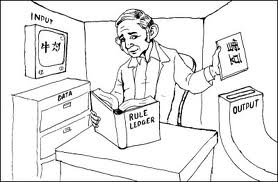
\includegraphics[width=.4\linewidth]{images/ChineseRoom.jpg}
		\caption[Searle's Chinese Room]{Searle's Chinese Room\footnotemark}
		\label{fig:ChineseRoom}
	\end{figure}\footnotetext{Image credits: \href{https://theness.com/neurologicablog/index.php/ai-and-the-chinese-room-argument/}{\texttt{https://theness.com/neurologicablog/index.php			/ai-and-the-chinese-
			room-argument/}}}
	
	Although this may seem like a pedantic distinction at first glance, the difference is truly important. The hypothesis that we can only ever simulate the ability to think is known as the weak AI hypothesis whereas the hypothesis that we can produce a machine capable of thought is the strong AI hypothesis \cite{Jones}. These both stand in contrast to Artificial General Intelligence, which is an intelligence capable of performing any intellectual task that a human can \cite{Buchanan}.
	
	\section{The History of Artificial Intelligence}
	
	
	One would think that artificial intelligence would have its roots in the last century or two, but mankind has dreamed of and proposed machines with human-like intelligence for thousands years, dating back to at least Homer \cite{Buchanan}. From our imagination and literature, artificial intelligence was brought into the realm of the academic by philosophers and mathematicians such as Ren\'e Descartes' ``mechanical man'' and Gottfried Wilhelm Leibniz's mechanical reasoning devices \cite{Buchanan}. Pascal and Leibniz both designed calculating machines capable of automated arithmetic, but proposing a calculator is far from what we think of as artificial intelligence today  \cite{Buchanan}.
	
	It was the rise of electronics from Turing, IBM, Bell Laboratories, and countless others in the mid-twentieth century started to change the question from a philosophical one to a practical one \cite{Buchanan}. Artificial intelligence is a testament to the kind of interdisciplinary problem solving encouraged by the liberal arts, with contributions coming from the fields such as engineering, biology, psychology, game theory, communication theory, logic, philosophy, and linguistics \cite{Buchanan}. Eventually, with advancements in computational power, operating systems, and language design, researchers were able to demonstrate impressive  computational problem solving such as Arthur Samuel's 1952 checker-playing program written in assembly language and one of the first examples of evolutionary computation \cite{Buchanan}. 
	
	Newell, Shaw, and Simon's ``Logic Theorist'' program became the first artificial intelligence written for a computer in 1956 \cite{Gugerty}. Through the use of heuristic algorithms, Logic Theorist was able to prove theorems and solve complex problems astonishingly well \cite{Gugerty}. These early attempts at artificial intelligence were largely doing two things: searching and finding ways to represent and manipulate knowledge. Claude Shannon pointed this out in his 1950 ``Programming a Computer for Playing Chess'' in which he produced what is now called the Shannon number, $10^{120}$, which is a lower bound of the game tree complexity of Chess \cite{Jones}.
	
	Artificial intelligence became formally recognized as a field of study and got its name from the 1956 Dartmouth Artificial Intelligence Conference \cite{Buchanan}. Another product of the conference was a step forward in artificial intelligence's ability to represent and manipulate knowledge with John McCarthy's development of the first AI programming language, LISP \cite{Jones}. The strides towards strong AI came crashing down with the publication of the 1969 paper ``Perceptrons'' which showed that single layer perceptrons were not able to properly handle linearly inseparable problems, leading to a steep decline in neural network research and ``AI Winter'' \cite{Jones}.
	
	Research into artificial intelligence reemerged in the mid to late eighties, but this time with a more practical focus rather than searching for Searle's strong AI \cite{Jones}. Algorithms developed and used for artificial intelligence found their way into camera auto-focus, anti-lock brakes, search engines, and medical diagnoses \cite{Jones}. Another marked difference is the plethora of approaches such as agent systems and biologically inspired systems. Today research into artificial intelligence has largely remained in this practical realm, using neural networks, data mining, fuzzy logic and other tools to solve real-world problems while slowly marching towards an Artificial General Intelligence.
	
	\section{Approaches to Intelligence}
	
	Artificial intelligence, because of how broadly the word can be defined and how many fields contribute the its progress, can be hard to wrap one's head around. However, Connell and Livingston have proposed four categories for artificial intelligence approaches which are useful for understanding the state of artificial intelligence research and the varied potential paths to Artificial General Intelligence \cite{Connell}.
	
	Their first category is labeled ``Silver Bullets'' and describes approaches in which much of what is needed is already believed to be present, but we are missing a crucial piece that will supposedly resolve our problems and deliver us a system with intelligence \cite{Connell}. Examples include `Fancy Logic' (second-order, non-monotonic, epistemic, deontic, modal, etc), Fuzzy Logic, Deep Language, Embodiment, and Quantum Computing \cite{Connell}. Disciples of this school of thought are chasing their particular ``Silver Bullet,'' working to formalize and perfect what they believe to be the missing link.
	
	They next describe the ``Core Values'' section which puts emphasis on the central organizational scheme over other computational details, believing that this macro-level structure has greater influence than the exact algorithms used \cite{Connell}. Situatedness, Emotionality, Self-Awareness, and Hierarchy \& Recursion are a few of these ideologies. There are strong arguments for this category, especially Hierarchy \& Recursions argument that an intelligence needs to be able to abstract recursively \cite{Connell}.
	
	Connell and Livingston's third category, ``Emergence,'' looks at artificial intelligence approaches which believe they already have the essentials, but we haven't implemented the essentials on a large enough scale to get our intelligence yet \cite{Connell}. For example, one might hold the position that intelligence is simply the ability to generate and search decision trees and we haven't realized an Artificial General Intelligence yet because our hardware doesn't allow us to do this effectively enough yet. Approaches in this category include Axiomatization, Commonsense, Learning, Evolution, and Integration \cite{Connell}.
	
	Lastly, we visit ``Emulation'' which is the school of thought that says we are better off copying intelligence than designing our own \cite{Connell}. Neural simulation, neural networks, animal models, human development, sociality, and cortical learning algorithms all fit in this category \cite{Connell}. The danger with this approach is abandoning theory in its sprint towards a functional copy, because if one does not understand the thing they have made, it is hard to see what it can do and where it can be improved. Another excellent point is that it can be very hard to correctly identify what needs to be copied, as Connell and Livingston note, ``artificial feathers and flapping turn out not to be needed to create airplanes'' \cite{Connell}.
	
	\section{Computational Neuroscience}
	
	Emulating natural processes--and even the human brain--is not a new idea to computer scientists. In fact, artificial neural networks that we still use today were originally proposed in a 1943 paper that introduced the first mathematical model of a neuron~\cite{FundNatComp}. The 1950's and 60's saw the rise of evolutionary computing which attempts to simulate evolution usually for finding optimal solutions to problems. Computational neuroscience is the newest field to emerge from this interdisciplinary intersection of biologists and computer scientists.
	
	\begin{figure}[!ht]
		\centering
		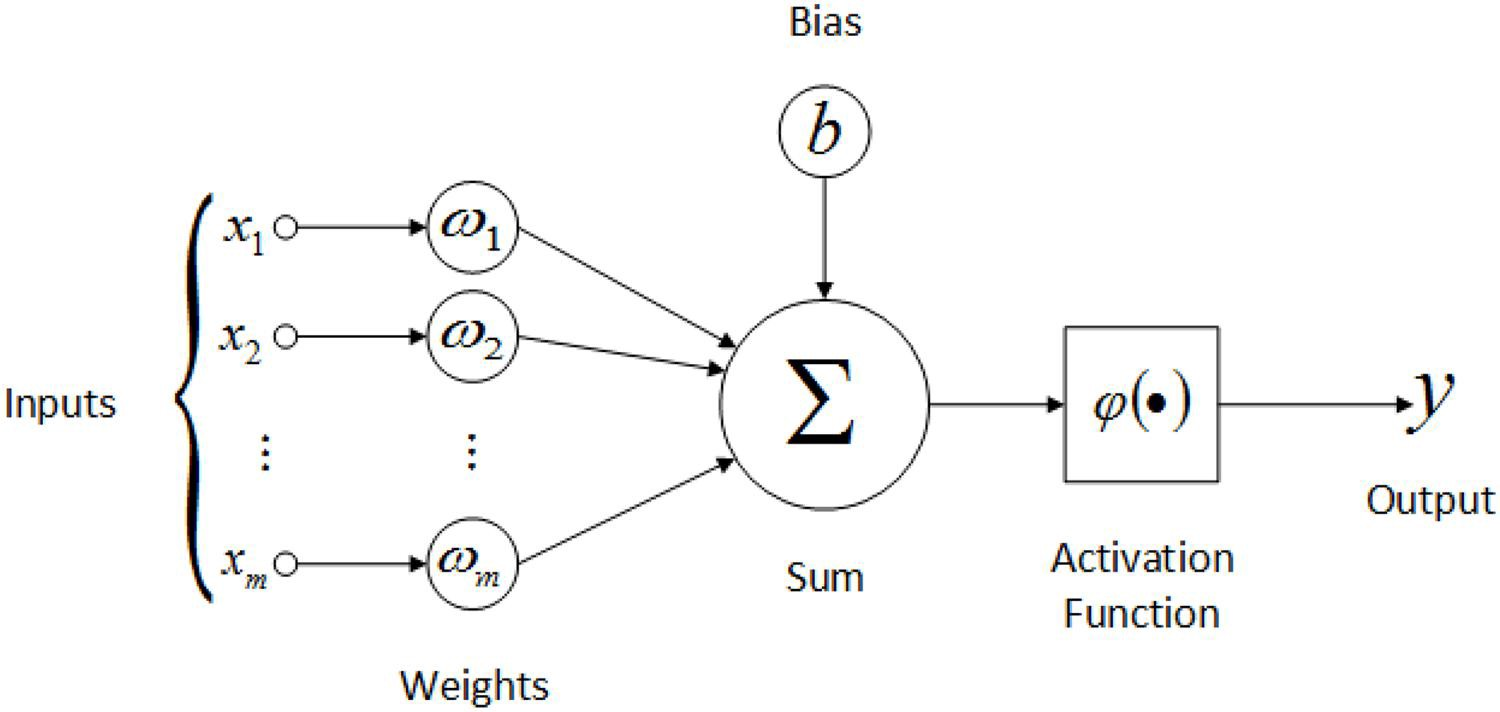
\includegraphics[width=.8\linewidth]{images/ArtificialNeuron.jpg}
		\caption{A Model for an Artificial Neuron}
		\label{fig:ArtNeuron}
	\end{figure}
	
	Computational neuroscience can be described as ``simulating human cognition using biologically based networks of neuronlike units''~\cite{Eberhart}. In other words, the field has tasked itself with the incredibly difficult task of trying to understand cognition by breaking the brain down into algorithms and data structures which we can then implement in a computational model. So rather than trying to create a computational model that is as intelligent as the brain, they are taking the more direct approach in attempting to model the brain itself.
	
	One such set of computational neuroscientists are the researchers at Numenta who are attempting to replicate the mammalian neocortex. Their founder, Jeff Hawkins, realized in the early 1980's that we needed to truly understand what made the brain intelligent before we created our own intelligence~\cite{OnIntelligence}. Unfortunately, this view was not shared by  researchers at Intel and MIT where he unsuccessfully attempted to start a research lab and study computer science respectively. To support his inquiry, Jeff Hawkins decided to supplement his computer science and engineering background with some training in biophysics and set out to develop a theoretical understanding of the neocortex. In 2002, he founded the Redwood Neuroscience Institute and Hawkins is currently developing cortical learning algorithms and Hierarchical Temporal Memory at Numenta which he founded in 2005~\cite{OnIntelligence}. 
	
	\chapter{Time Series}
	
	A \textbf{time series} is a ``sequence of observations taken sequentially in time'' and are everywhere in today's world~\cite{Box}. Figure~\ref{fig:TimeSeriesExamples} shows two such examples, stock prices (Figure~\ref{fig:AMDChart}) and levels of precipitation in Seatle, WA from 1948-1979 (Figure~\ref{fig:SeattlePrecip}). Their ubiquity drives a desire to understand, characterize, and predict time series, but it can be an extremely complex task because there is generally a dependence on prior terms due to the sequential nature and some uncertainty to their movements.
	
	\begin{figure}[!ht]
		\centering
		\begin{subfigure}[b]{.45\textwidth}
			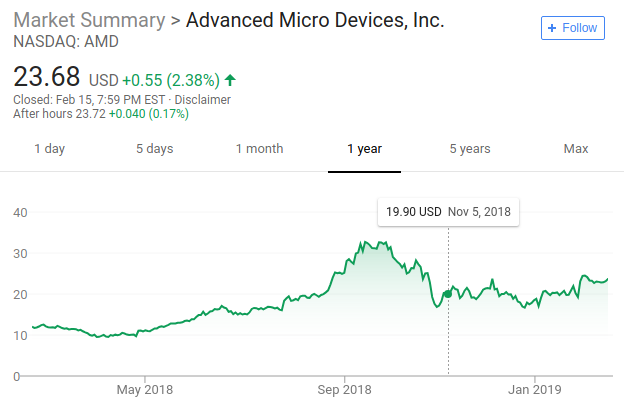
\includegraphics[width=\textwidth]{images/AMDChart.png}
			\caption{A chart of AMD stock prices}
			\label{fig:AMDChart}
		\end{subfigure}
		\begin{subfigure}[b]{.45\textwidth}
			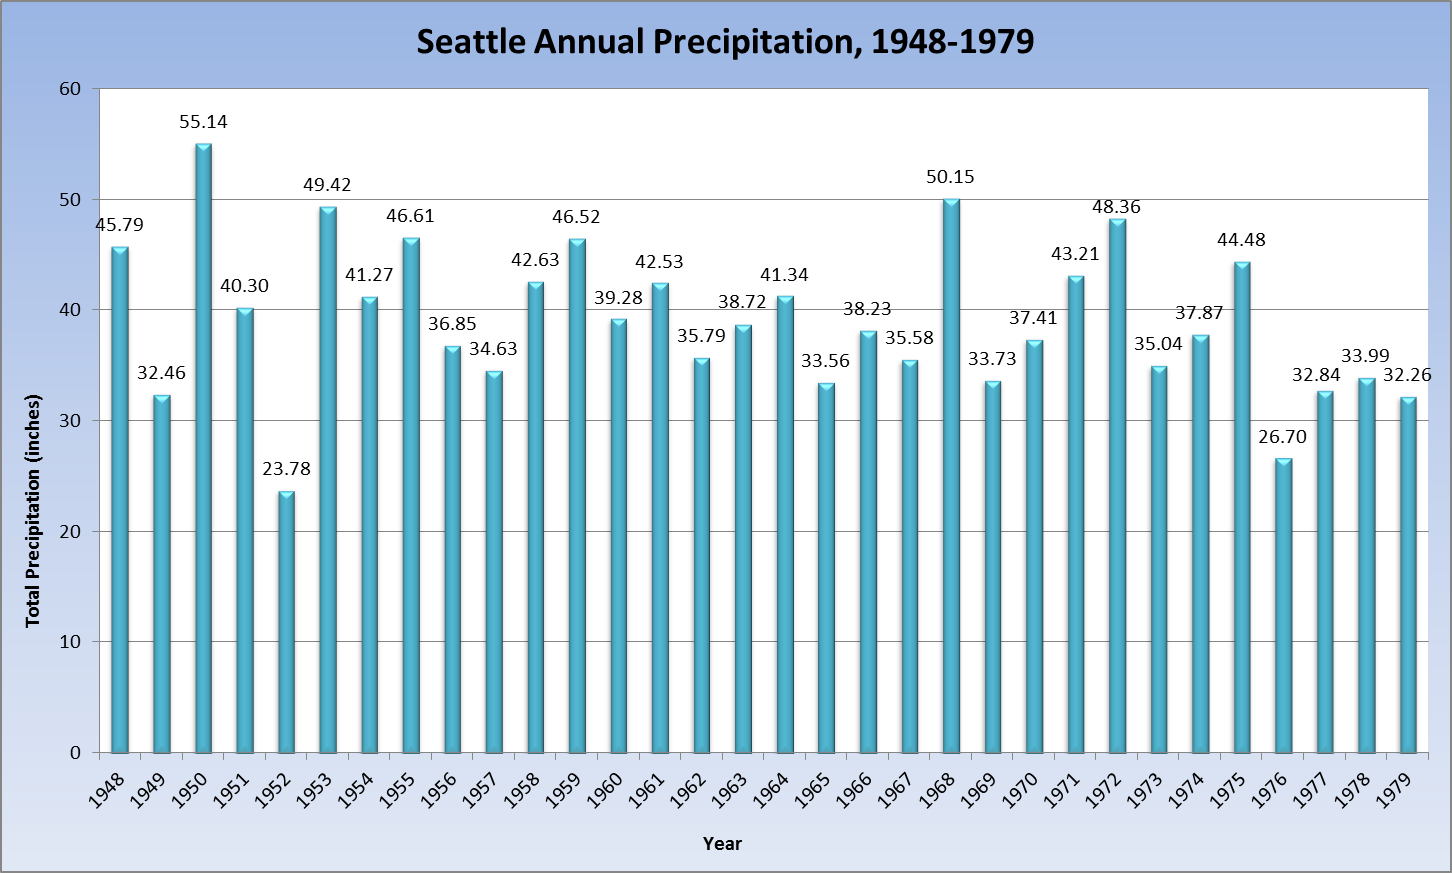
\includegraphics[width=\textwidth]{images/SeattleRainfall.png}
			\caption{Seattle precipitation, 1948-1979}
			\label{fig:SeattlePrecip}
		\end{subfigure}
		\caption[Examples of Time Series]{Examples of Time Series \footnotemark}
		\label{fig:TimeSeriesExamples}
			
	\end{figure}
\footnotetext{Image (b) courtesy of Seattle Weather Blog: \href{http://www.seattleweatherblog.com/rain-stats/}{\texttt{http://www.seattleweatherblog.com/rain-stats/}} }

	\section{Autoregressive Models}

	 One model for representing time series is the autoregressive (or AR) model. In an autoregressive model, the series at some time $t$ is expressed as a finite weighted sum of previous values of the series plus a random component $a_{t}$~\cite{Box}. Let $z_{t}, z_{t-1}, z_{t-2},...$ denote the series at times $t, t-1, t-2,...$. Further, let $\mu$ be the mean or level of the process and let $\tilde{z}_{t-n}=z_{t-n}-\mu$. We can then express an autoregressive process of order $p$ by
	
	\begin{align}
		\label{eqn:armodel}
		\tilde{z}_{t}=\phi_{1} \tilde{z}_{t-1}+\phi_{2} \tilde{z}_{t-2}+...+\phi_{p} \tilde{z}_{t-p}+a_{t}
	\end{align}
	
	\noindent where $\mu, \phi_{1}, \phi_{2}, ..., \phi_{p}, \sigma^{2}_{a}$ are the $p+2$ unknown parameters of the model with $\sigma^{2}_{a}$ being the variance of the white noise process $a_{t}$~\cite{Box}. Using a backshift operator $B$ such that $Bz_{t}=z_{t-1}$ we can define an autoregressive operator of order $p$ by
	
	\begin{align}
		\label{eqn:arop}
		\phi(B)=1-\phi_{1}B-\phi_{2}B^{2}-...-\phi_{p}^{p}
	\end{align}
	
	\noindent which allows us to write an autoregressive model succinctly as $\phi(B)\tilde{z}_{t}=a_{t}$~\cite{Box}.

	\section{Moving-Average Models}
	
	Suppose instead that the true process is regressed on the random shocks rather than the deviations from the level. Starting from our autoregressive model  of order p we can recursively substitute the model's definition of $\tilde{z}_{t-n}$ until we end up with an infinite summation of innovation terms~\cite{Box}. However, the moving average model provides us a much more direct approach by representing the time series as a finite number of shocks to the process. Formally we express a moving average (MA) model of order $q$ by
	
	\begin{align}
		\label{eqn:mamodel}
		\tilde{z}_{t}=a_{t}-\theta_{1}a_{t-1}-\theta_{2}a_{t-2}-...-\theta_{q}a_{t-q}
	\end{align}
	
	\noindent just as with the autoregressive model, we have $q+2$ unknown paramters and using the backshift operator we can define a moving average operator that allows us to express the model more succinctly yielding $\tilde{z}_{t}=\theta(B)a_{t}$~\cite{Box}.

	\section{Autoregressive Moving-Average Models}
	
	Real world processes may require a combination of these two approaches for a succinct and accurate model, resulting in a mixed Autoregressive Moving-Average (ARMA) model~\cite{Box}. Such a model includes terms from both the autoregressive and moving average model resulting in:
	
	\begin{align}
		\label{eqn:armamodel}
		\tilde{z}_{t}=\phi_{1} \tilde{z}_{t-1}+...+\phi_{p} \tilde{z}_{t-p}+a_{t}-\theta_{1}a_{t-1}-...-\theta_{q}a_{t-q}
	\end{align}
	
	\noindent This model has $p+q+2$ unknown parameters and can also be written more succinctly using our autoregressive operator and moving average operator resulting in $\phi(B)\tilde{z}_{t}=\theta(B)a_{t}$~\cite{Box}.

	\section{Classification of Time Series}\label{sec:timeseries:classification}

	A key question in time series analysis is how to select the correct model for a given time series. There are a few approaches, but one is to use information criterion such as the Akaike Information Criterion or the Bayes Information Criterion~\cite{Box}. For both AIC and BIC, optimal models minimize the information criterion and there is a penalty for the number of parameters used resulting in a bias towards a smaller set of parameters. The formula for BIC is

	\begin{align}
		\label{eqn:bic}
		BIC_{p,q}=\ln(\hat{\sigma}_{a}^{2})+r\frac{\ln(n)}{n}
	\end{align}

	\noindent where $n$ is the sample size, $\hat{\sigma}_{a}^{2}$ is the maximum likelihood estimate of $\sigma_{a}^{2}$, and $r=p+q+1$ is the number of parameters estimated in the model.
	
	The ubiquity of time series makes forecasting them an important and many times profitable task such as in the case of financial time series (as seen in Figure~\ref{fig:AMDChart}), making them a common prediction task for machine learning and artificial intelligence systems. It allows us to test an ``intelligent'' systems ability to discover temporal patterns which may sometimes be fuzzy or complex: a hallmark of human intelligence.
	
	
	
	
	
	
	
	\chapter{Biologically Inspired Computing}
	
	\section{Particle Swarm Optimization}
	
	Introduced in by Russell Eberhart and James Kennedy in their 1995 paper, \textit{A New Optimizer Using Particle Swarm Theory}, Particle Swarm Optimization has changed the way the world optimizes continuous nonlinear functions~\cite{PSOReview}. Swarming is fast and effective for optimization over complex multidimensional search spaces and lends itself well to parallelization due to its multi-agent approach, making it an excellent choice for optimizing parameters in neural networks and is implemented by Numenta for finding optimal parameters.
	
	Usually abbreviated to PSO or \textit{swarming}, it draws inspiration from bird flocks and schools of fish~\cite{Eberhart}. The concept is quite simple: it simulates particles on parameter space and at each time-step every particle evaluates fitness as a function of its location in parameter space, then moves towards some linear combination of its personal best and the overall best score among the particles using weights representing a cognitive constant or individuality (denoted $c$) and a social constant (denoted $s$).
	
	\begin{figure}[!ht]
		\centering
		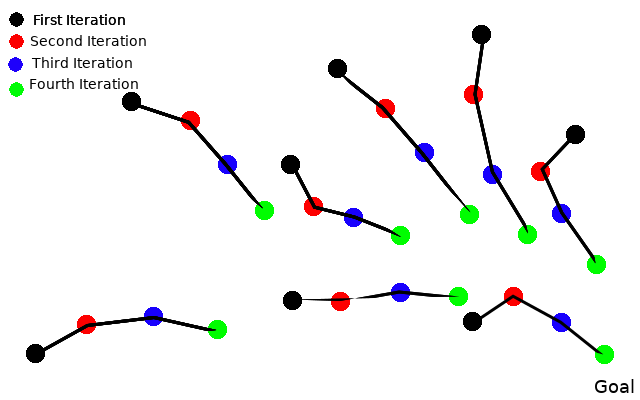
\includegraphics[width=.7\linewidth]{images/PSOVisual.png}
		\caption{Visualization of the PSO Algorithm}
		\label{fig:PSOVisual}
	\end{figure}
	
	The algorithm begins by initializing all particles with a random coordinate in the parameter space and a random velocity. Then at each time step, it calculates its fitness based on the function being optimized and the parameters associated with its position in parameter space. If this fitness is the best the particle has achieved, it is recorded as its personal best, denoted \texttt{pbest} and the particle with the best fitness is chosen as global best, denoted \texttt{gbest}. We then update the velocity and particle position of each particle in our swarm using the equations described in Equation~\eqref{eqn:psoupdate} where $v_{t}$ is the velocity of a particle at time step $t$, $p_{t}$ is the position of a particle at time step $t$, and $\beta_{1}, \beta_{2}$ are uniformly distributed random variables with $\max(\beta)$ being a parameter of the algorithm~\cite{PSOReview}.
	
	\begin{align}
	\label{eqn:psoupdate}
	\begin{split}
	v_{t+1} &= v_{t}+c\times \beta_{1} \times (\text{pbest}-p_{t})+s\times \beta_{2} \times (\text{gbest}-p_{t}), \\
	p_{t+1} &= p_{t} + v_{t+1} .
	\end{split}
	\end{align}
	
	I utilized swarming to find optimal or near-optimal sets of parameters for learning ARMA time series with a Hierarchical Temporal Memory network. Numenta themselves utilizes swarming for this very same purpose, and NuPiC comes with a swarming utility, however I wrote my own swarming utility in Python which I thoroughly tested on a number of complex surfaces.
	
	\section{Hierarchical Temporal Memory}
	
	Hierarchical Temporal Memory is a framework attempting to produce cortical learning algorithms---algorithms that mimic the processes of the human neocortex. In the human brain, the neocortex is approximately seventy-percent of the brain's volume~\cite{DiscoveriesBrainWorks}. It can be described as a ``wrinkly sheet of sheet of cells, about two millimeters thick'' and is responsible for the characteristics of intelligence that set humanity apart from other species~\cite{DiscoveriesBrainWorks}. 
	
	\begin{figure}[!ht]
		\centering
		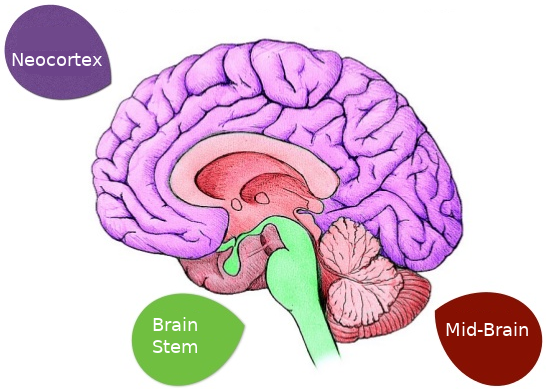
\includegraphics[width=.5\linewidth]{images/Brain.png}
		\caption{Overview of the Human Brain}
		\label{fig:brain}
	\end{figure}
	
	For all of its complexity, the neocortex has an incredibly consistent microarchitecture of cortical columns which are in turn made up of neurons~\cite{DiscoveriesBrainWorks}. Neuroscientist Vernon Mountcastle revolutionized the way we think about our own brains when he proposed that the consistent architecture must imply consistent processes across the cortex. This would mean that all of our high-level thinking must essentially be the same on the level of the cortical column. Therefore if we can understand how a cortical column functions, we can understand the entire cortex~\cite{DiscoveriesBrainWorks}.	
	
	\begin{figure}[!ht]
		\centering
		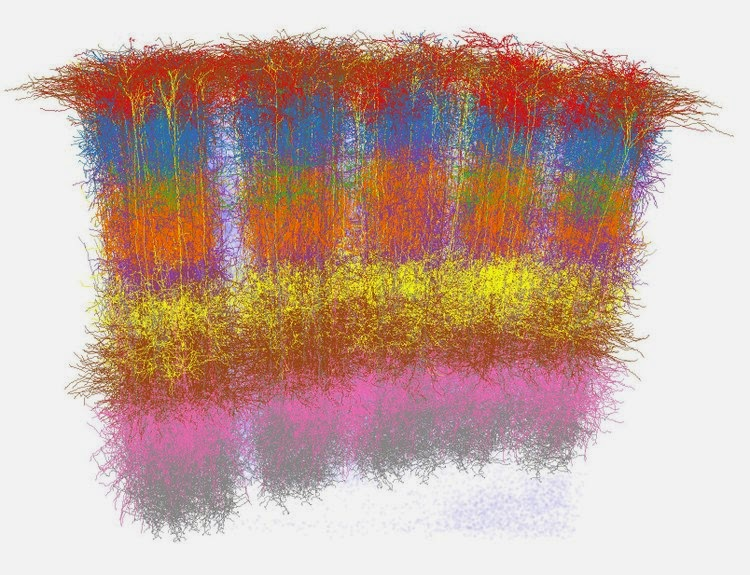
\includegraphics[width=.6\linewidth]{images/CorticalColumns.jpg}
		\caption[3D reconstruction of five neighboring columns in rat vibrissal cortex]{3D reconstruction of five neighboring columns in rat vibrissal cortex\footnotemark}
		\label{CorticalColumn}
	\end{figure}\footnotetext{Image credit: Marcel Oberlaender et al.}
	
	\subsection{Sparse Distributed Representations}\label{sec:sdr}
	
	A key to understanding how the brain functions is understanding how the brain perceives the world. Our senses need to be encoded into a common language that is compatible with the circuitry of the cortex, and understanding how that process works is an enormous challenge itself. As an example, consider the field of Natural Language Processing. It is a field that has had an enormous amount of work done for decades and yet NLP is still incapable of human-like interpretation of text. One system of encoding that hopes to provide a language for cortical circuitry is sparse distributed representations.
	
	Consider the binary representation of the integer 16 versus that of the integer 15. The two numbers are quite similar: they are only 1 apart, so they are as close as two integers can be. Yet their binary representations are [100000] and [011111] respectively. They have no shared ``on'' bits so despite their similarity, their binary representations reflect none at all. In fact, despite being as close as two integers can be (a Euclidean distance of 1), their binary representations have a Hamming distance, the number places in which two codewords differ, of 5, the maximum Hamming distance of two codewords of length 5 \cite{Adams}. 
	
	This means that our encoding does not preserve semantic similarity or a concept of distance between elements which is highly undesirable for an code because if there is some kind of error in the code we could end up decoding something meaning the opposite of what we were trying to convey. As an example, consider $\mathbb{Z}$ from 0 to 31 which is mapped to $GF(2)^{6}$ by their binary representation. The mapping of 31 is [111111] but a single error in transmission can easily lead to [011111] which would be decoded as 15. So a code Hamming distance ($d_{H}$) of one away ($\frac{1}{5}$ of the total metric) lead to an element 16 integers away ($\frac{1}{2}$ of the total metric). We would obviously like to avoid this so that errors in the transmission of our codes are either (1) correctable or (2) lead to a decoding that is as close as possible to our original element.
	
	This is achievable by simply conveying more information in our code. In our binary representation any single error led to another valid codeword (a codeword which decoded to an element of the input/output set) which meant that no errors could be detected or corrected. By expanding our code length, we increase the number of codewords (multiplying by the cardinality of the code alphabet for each character added) meaning that fewer errors will result in other valid codewords and can possibly be detected or corrected. 
	
	A key strategy with Sparse Distributed Representations is to encode semantic similarity, such as with our idea of distance in our motivating example. This helps us achieve our second goal because even if we increase the error-tolerance of our code, there is still some probability of an uncorrectable error and we would like that error to result in a codeword as close to the original codeword as possible. To give you a real world example imagine I am sending instructions to a aircraft and I need to tell it to turn down 7\textdegree~to start its descent. Obviously, an error resulting in 8\textdegree~or 6\textdegree~being interpretted by the pilot are both preferable to 90\textdegree.
	
	To achieve our goal, we employ sparse distributed representations or SDRs. Just as with traditional dense binary representations, we will represent sparse distributed representations as vectors over their code alphabet, in this case GF(2). We call them \textbf{sparse} distributed representations because these vectors typically only have a small proportion of the components as 1. We will use Numenta's notation of letting $w_{\overrightarrow{x}}$ denote the number of components in an SDR $\overrightarrow{x}$ that are 1, so $w_{\overrightarrow{x}} = \norm{x}_{1}$ \cite{Properties}.
	
	Given our definition of distance, we could say that two decodings of sparse distributed representations, $a$ and $b$, are equal if and only if the $d_{H}(a,b) = w_{a} = w_{b}$. This would mean that both vectors would have to have the same dimensionality, same number of on bits, and all on and off bits would have to match. This definition is good for ``equals,'' but suppose we have a single error in transmission or a single component of our distributed system fails, equality would thus fail. In order to be able preserve the ability to subsample and thus to preserve fault tolerance, we therefore need a less stringent definition for decoding SDRs. Numenta refers to this as the $overlap$, which is 
	
	\begin{align}
	\label{eqn:overlap}
		overlap(\overrightarrow{a}, \overrightarrow{b}) \equiv \overrightarrow{a} \cdot \overrightarrow{b} \equiv \sum_{0}^{n-1} a_{i}b_{i}
	\end{align}
	
	
	 Thus, we say two SDRs $\overrightarrow{a}$ and $\overrightarrow{b}$ decode to the same element of the input space if and only if $overlap(a,b) \geq \theta$ where $\theta \leq w_{a}$ and $\theta \leq w_{b}$ \cite{Properties}. Denote the function that determines if two sparse distributed representations decode to the same element of the input space using some $\theta$ and $overlap(\overrightarrow{a}, \overrightarrow{b})$, $match_{\theta}(\overrightarrow{a}, \overrightarrow{b})$ and it is a function from SDR$\times$SDR $\longrightarrow$\{true, false\}.
	
	Given a set of sparse distributed representations with the same dimension, $X =\{\overrightarrow{x_{1}}, \overrightarrow{x_{2}}, ...,\overrightarrow{x_{n}}\}$, we can union the vectors using the bitwise OR operation over the $i^{th}$ position of the vectors in the set to produce the $i^{th}$ position of $union(X)$ \cite{Properties}. For example, given [0100] and [0010] the union would be [0110]. We say an SDR $\overrightarrow{y}$ is an element of the union of a set of SDRs, $\overrightarrow{X}$, if and only if $match_{\theta}(\overrightarrow{X},\ \overrightarrow{y})$ \cite{Properties}.
	
	\subsection{Cortical Learning Algorithms}
	
	Hierarchical Temporal Memory aims to implement the functions of the neocortex as faithfully as possible, and unsurprisingly uses the same atomic unit of the cell. Modeled after the pyramidal neurons of the neocortex, these cells each take their own inputs and make their own predictions which the layer combines into a cohesive prediction \cite{Whitepaper}. They have three states: active from feed-forward input, active from lateral input (predictive state), and inactive. These first two states correspond to a short burst of action potentials in a neuron, and a slower steady burst of action potentials on a neuron respectively in our own brain.
	
	\begin{figure}[!ht]
		\centering
		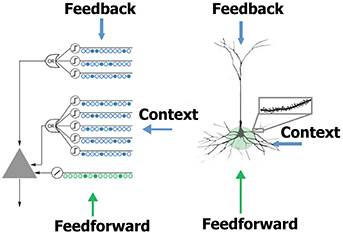
\includegraphics[width=.7\linewidth]{images/HTMCell.jpg}
		\caption[Pyramidal Neuron vs. Hierarchical Temporal Memory Cell]{Pyramidal Neuron vs. Hierarchical Temporal Memory Cell~\cite{TheHTMSpatialPooler}}
		\label{fig:HTMCell}
	\end{figure}

	Just like actual pyramidal neurons, HTM cells also dendrite segments. Each cell has one proximal dendrite segment and a dozen or more distal dendrite segments \cite {Whitepaper}. Proximal dendrites accept feed-forward input and all cells in the same column respond to a similar feed-forward input due to a class of inhibitory cells. On the other hand, distal dendrites receive lateral input from nearby cells and their response is unique on a cell-by-cell basis dependent on the connected synapses on each cells distal dendrites~\cite{Whitepaper}. Figure~\ref{fig:HTMCell} illustrates the similarities between a pyramidal neuron and an HTM cell.
	
	In a biological neuron synapses have real number weights with a stochastic nature, but in the HTM model synapses have binary weights (connected or disconnected) that are informed by real number permanence values~\cite{Whitepaper}. These permanence values allow our artificial neurons to model forming and un-forming of ``potential synapses'' which represent axons that pass close enough to a dendrite segment that they could potentially form a synapse. Once the permanence is above a certain threshold (a parameter of the network) the synapse is considered connected.
	
	\subsubsection{Encoder}
	
	As discussed in Section~\ref{sec:sdr}, in the real world we need to encode sensory data to a format which the cortex can understand. The entire data pipeline of Hierarchical Temporal Memory can be seen in Figure~\ref{fig:HTMpipeline}. For numeric data, we generally use a Random Distributed Scalar Encoder. Just as with any scalar encoder, it is a function from a number to a binary vector with \texttt{width} 1 bits and the rest of the bits being zero. All scalar encoders also have either implicitly or explicitly a \texttt{resolution} parameter which determines the size of the ``buckets'' in which all numbers in that ``bucket'' are encoded to the same binary vector, this is essentially the lower-limit topology on $\mathbb{R}$. This is necessary because for a binary vector of length $n$ there are only $2^{n}$ possibly options and infinite real numbers between any two numbers.
	
	\begin{figure}[!ht]
		\centering
		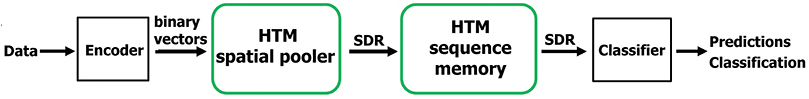
\includegraphics[width=\linewidth]{images/DataPipeline.jpg}
		\caption[Data Pipeline of an HTM]{Data Pipeline of an HTM~\cite{TheHTMSpatialPooler}}
		\label{fig:HTMpipeline}
	\end{figure}

	A region's input space and output space are the same; an HTM takes in a time series over the space and predicts an element or set of elements of the input space it believes to come next \cite{Purdy}. Each region has an input space which could be a single input set or the Cartesian product of multiple input sets. As an example, \{0,1,2,3,4\} could be an input set and if a parent region receives input from child region which has \{0,1\} as its input space and another child region with \{red, green, blue\} as its input space, then the parent region's input space would be \{(0, red), (1, red), (0, green), (1, green), (0, blue), (1, blue)\}. An encoding function from an input space to $n$-dimensional sparse distributed representations is not guaranteed to be surjective or injective. We would not expect surjectivity, but could get it through nearest neighbor decoding, but injectivity is something that one would think would be preserved. However, because parent regions are allowed to take a slice of the output vector (not the ``on'' bits, just an arbitrary portion) when being fed to from multiple child regions, we cannot guarantee the property.
	
	\subsubsection{Spatial Pooler}

	The Spatial Pooler's job is to receive the encoded representation of the input space and convert the input to a sparse pattern-a requirement for learning and prediction in Hierarchical Temporal Memory theory~\cite{Whitepaper}. Upon initialization, all of the potential synapses on the dendrite segments of all of the mini-columns are randomly assigned permanence values and based on these permanence values a potential synapse may be valid or not~\cite{Whitepaper}. 

	\begin{figure}[!ht]
		\centering
		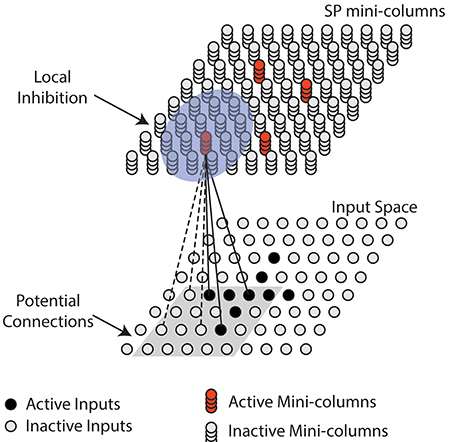
\includegraphics[width=.6\linewidth]{images/SpatialPooler.jpg}
		\caption[Spatial Pooler]{Spatial Pooler \cite{TheHTMSpatialPooler}}
		\label{fig:SpatialPooler}
	\end{figure}

	
	The pooler begins with an input from the encoder that has a fixed number of bits and for each column we determine how many valid synapses are connected to active input bits~\cite{Whitepaper}. This number is then multiplied by a ``boosting'' factor determined dynamically by how often a column is active relative to its neighbors. The most highly activated mini-columns after boosting then disable a percentage of the mini-columns within a dynamically determined ``inhibition radius'' to create a sparse set of activated mini-columns~\cite{Whitepaper}. Lastly, each active column updates the permanence values of its potential synapses. The permanence values associated with active input bits are increased while those associated with inactive bits are decremented~\cite{Whitepaper}.

	
	\subsubsection{Temporal Pooler}

	The temporal pooler takes over where the spatial pooler left off, with a sparse set of activated mini-columns. For each active mini-column, if there are cells in the predictive states, activate them and in the absence of a cell in the predictive state, activate all of the cells in the mini-column~\cite{Whitepaper}. The set of active cells is the HTM's representation of the current input in the context of the previous of the previous inputs~\cite{BAMI}. Next, each cell's dendrite segment counts how many connected synapses are associated with active cells and if this number is above a certain threshold, the dendrite segment is activated. A cell with an active dendrite segment is put into a predictive state in the next time step~\cite{BAMI}. The algorithm is illustrated in Figure~\ref{fig:TemporalPooler}.
	
	

	\begin{figure}[!ht]
		\centering
		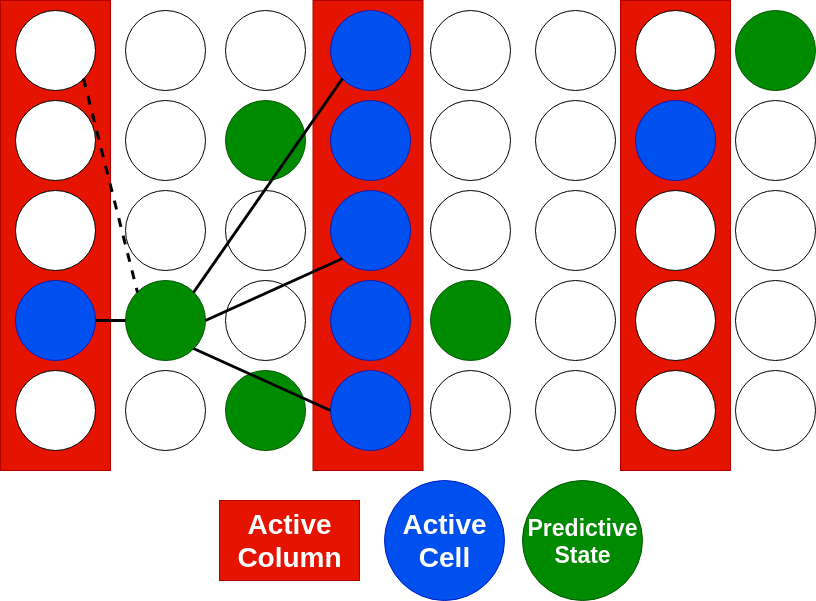
\includegraphics[width=.8\linewidth]{images/TemporalPooler.png}
		\caption{Temporal Pooler}
		\label{fig:TemporalPooler}
	\end{figure}

	\subsubsection{Classifier}
	
	Once the system completes its processing of a time step's input, the system outputs a sparse distributed representation which may have gone through multiple layers and it is important to be able to decode the system's prediction in order for the system to be useful. Hierarchical Temporal Memory currently uses something called an SDR Classifier to decode the predictions of an HTM \cite{Dillon}. At its essence, an SDR Classifier is a single layer, feed forward, neural network \cite{Dillon}.
	
	\begin{figure}[!ht]
		\centering
		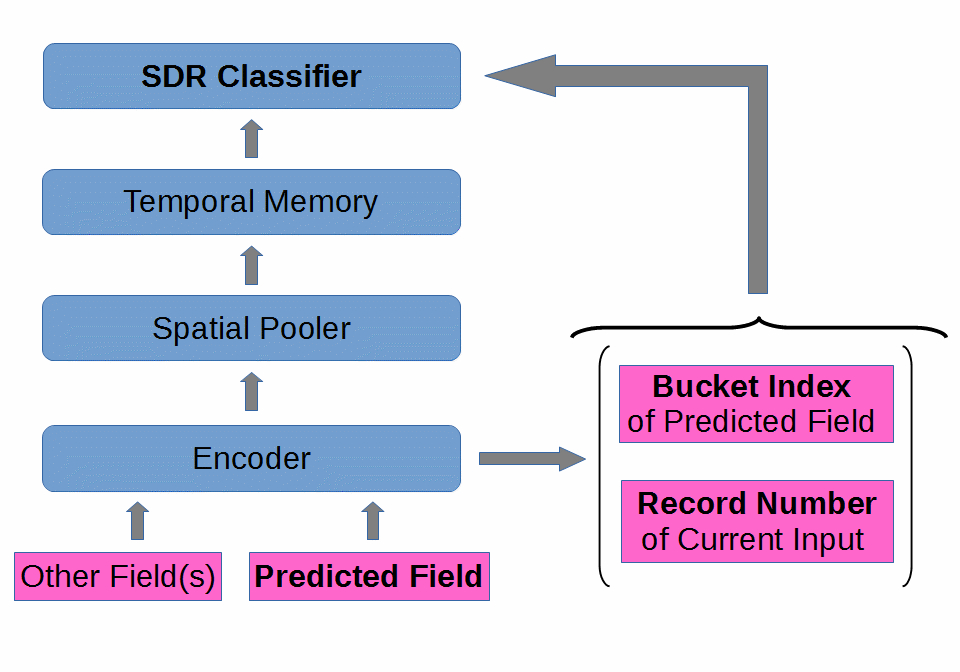
\includegraphics[width=.6\linewidth]{images/SDRClassifier.jpg}
		\caption{SDR Classifier}
		\label{fig 3}
	\end{figure}
	
	SDR Classifiers are able to decode the information HTMs give about predictions $n$ times steps in the future by maintaining a weight matrix \cite{Dillon}. The matrix's weights are adjusted to ``learn'' after each time step to reflect the correct weighting between the output vector at time $t$ and the probability distribution of the input/output space at time $t-n$ \cite{Dillon}. This enables the matrix to reflect relationships between inputs and outputs $n$ time steps apart. To determine the SDR Classifier's interpretation of an output at time $t+n$, the SDR Classifier takes in the HTM's output vector and uses Softmax to determine the most likely decoding \cite{Dillon}. So for each of the $k$ classes in the output space, the certainty that the output vector is referring to it is 
	
	\begin{align}
	\label{eqn:htmclassact}
	y_{j} = \dfrac{e^{a_{j}}}{\sum_{i=1}^{k} e^{a_{i}}}
	\end{align}
	
	
	 \noindent where $a_{j}$ is the activation level of the $j^{th}$ element of the output space, calculated by multiplying the output vector by the $j^{th}$ column of the weight matrix element wise \cite{Dillon}. 
	
	\chapter{Literature Review}
	
	
	There has been some work in evaluating Hierarchical Temporal Memory's ability to predict time series. Numenta themselves has published a paper, \textit{Evaluating Real-Time Anomaly Detection Algorithms - the Numenta Anomaly Benchmark} in which they showed that the HTM algorithm outperformed other tested anomaly detectors for streaming data~\cite{NAB}. Their anomaly detection is also the center-piece of a number of applications on their HTM applications website\footnote{\href{https://numenta.com/machine-intelligence-technology/applications/}{\texttt{https://numenta.com/machine-intelligence-technology/applications/}}} listing ``rogue behavior'' detection, geospatial tracking, and financial monitoring services. The IT analytics company Grok is another commerical application of HTM anomaly detection and is a partnership between Avik Partners and Numenta.
	
	Outside of Numenta's work, there have been a few studies done on an HTM's ability to predict time series, two of which focused on financial time series. The first of these found ``A fair amount of the generated models reached the goal of at least a 1.05 TP/FP ratio, and several models also made a profit''~\cite{Evaluation}. However, the author also noted, ``there was more room for improvements through either larger models or...through parameter optimization...''~\cite{Evaluation}. Gabrielsson et. al. built on this work and found that ``results show that HTM models outperformed the neural network models,'' but possibly more interestingly found that ``even though the number of bad trades (False Positives) outnumber the number of good trades (True Positives) in both the validation- and test sets, all models still yielded positive PNLs [Profits Net Losses]''~\cite{EvolvingTrading}. This could indicate that HTMs are not outperforming in terms of all prediction, simply anomaly prediction.
	
	Two contrasting views are found in papers that more directly looked at the time series capabilities of Hierarchical Temporal Memory. The first, a Master's Thesis by Michael Galetzka, asked an HTM to predict the navigation behavior of visitors to a website using publicly available data from \texttt{msnbc.com}~\cite{Galetzka}. The paper found that the HTM had a ``surprisingly high'' prediction accuracy for the kind of noisy data it was given and claims that the results are comparable or better than state-of-the-art approaches, but acknowledges that comparisons are difficult due to a lack of a uniform performance metric across papers.
	
	Most relevant to this exploration of ARMA models is Vivmond's \textit{Utilizing the HTM algorithms for weather forecasting and anomaly detection}. This paper applied HTMs to weather time series such as wind direction, wind speed, wind pressure, precipitation, humidity, and temperature some of which are quite literally textbook examples of ARMA models~\cite{Box,WeatherForecast}. Vivmond found that `` its prediction results were for the most part outperformed by a much simpler analogue method that used the average of the last few days as its forecast basis''~\cite{WeatherForecast}. 
	
	In particular, he points to Hierarchical Temporal Memory's inability to generalize trends, saying ``it is largely useless when seeing new values or when seeing previously seen patterns with different values''~\cite{WeatherForecast}. Vivmond also points to why he believes this is the case stating, ``if NuPIC was to learn a pattern consisting of several numbers and then be given a series of new numbers arranged in a similar pattern to the previous one, but with either higher, lower, or stretched values (i.e. multiplied by common a factor), it would be unable to correctly predict any of them''~\cite{WeatherForecast}. Although it is unclear if he tested this or not, the it fits with the theory of Hierarchical Temporal Memory because entirely different columns would be representing the numbers and the cells in those columns would have to re-form connections to each other in order to relearn ``new'' the pattern.
	
	
	
	
	
	\chapter{Experiment Design}
	
	\section{Hardware and Software Specifications}
	
	I utilized the official Python (Python 2.7) implementation of Numenta's cortical learning algorithms, NuPIC\footnote{NuPIC repository: \href{https://github.com/numenta/nupic}{\ttfamily https://github.com/numenta/nupic} } and it's Network API\footnote{Network API docs: \href{http://nupic.docs.numenta.org/stable/api/network/}{\ttfamily http://nupic.docs.numenta.org/stable/api/network/}}. At the time of my work NuPIC was at version 1.05 and I chose to use this version. It should be noted that although much of NuPIC is in Python, many of its computationally intensive algorithms are implemented in C++ using their NuPIC.core repository\footnote{NuPIC.core repository: \href{https://github.com/numenta/nupic.core}{\ttfamily https://github.com/numenta/nupic.core}} and it also relies on a number of external libraries such as \texttt{numpy} and \texttt{pandas}. 
	
	Due to the computationally intensive nature of my research and the limited time available to me, I also heavily relied on parallel processing to run my code in a reasonable time frame. In particular, the \texttt{multiprocessing} package in Python was indispensable to my research, allowing me to speed my code up a factor of up to 28x when running independent tests or swarming.
	
	\begin{table}[!ht]
		\centering
		\begin{tabular}{|l|l|}
			\hline
			\multicolumn{2}{|l|}{\textbf{Dijkstra (Asus Vivobook)}} \\ \hline
			CPU     & Intel i5-8250U, 4-Core, 1.60GHz     \\ \hline
			RAM     & 24 GB                                \\ \hline
			OS      & Linux Mint 19 Cinnamon               \\ \hline
			\multicolumn{2}{|l|}{\textbf{Galois (HP DL380 G7)}}     \\ \hline
			CPU     &  2x Intel Xeon X5650, 6-Core, 2.70 GHz       \\ \hline
			RAM     & 192 GB                               \\ \hline
			OS      & Linux Mint 19 Cinnamon               \\ \hline
			\multicolumn{2}{|l|}{\textbf{Aslan (HP DL380 G9)}}                         \\ \hline
			CPU&    2x  Intel Xeon E5-2690, 10-Core, 3.00 GHz    \\ \hline
			RAM&    256 GB                                  \\ \hline
			OS&    Gentoo                               \\ \hline
		\end{tabular}
		\caption{Hardware Specifications}
		\label{tab:hardware}
	\end{table}

	On the hardware side of things, the majority of development and testing was conducted on my personal laptop, an Asus Vivobook with some small upgrades. The code was then deployed to Aslan or Galois which had more cores, more memory, and a higher clock speed allowing me to get faster results. For a synopsis of the hardware specifications, see Table~\ref{tab:hardware}. 
	
	\section{Training Routine}\label{sec:exp:train}
	
	Our proposed exploration of how well a Hierarchical Temporal Memory network is able to predict ARMA models requires that we are able to train an HTM network. This required a flexible training routine that would allow us to train an HTM on a variety of of different sequences which may require vastly different parameters. 
	
	To do this, we drew on the training techniques of typical machine learning algorithms: we divided our data (in our case a sample from an ARMA model) into a training set, a validation set, and an evaluation set. Before an HTM enters the classical training however, we added a phase before that in which the spatial pooler could encounter the data without the temporal pooler being turned on. We hoped this would allow the spatial pooler to form some of its synapses before turning on the temporal pooler and thus have the temporal pooler learn on less ``noise.''. The number of iterations was a parameter we tuned\footnote{tuned through swarming\label{footnote:swarm}} called \texttt{sibt} (\textbf{S}patial pooler \textbf{I}terations \textbf{B}efore \textbf{T}emporal pooler).
	
	Then the classical machine learning techniques kicked in with the HTM learning its test set, then being tested on its validation set until performance stagnated or worsened, at which point we tested the HTM on the evaluation set. There are a few small differences in that we added a \texttt{iter\_per\_cycle} parameter\textsuperscript{\ref{footnote:swarm}} which allowed us to run on the test and validation set multiple times, summing the performances, before comparing to the previous, which would be useful for dealing with noise in the performance metric. We also added a \texttt{max\_cycles}\textsuperscript{\ref{footnote:swarm}} parameter that acted as a cut-off switch, stopping training after that many cycles. Most importantly, a weighting scheme as added (\texttt{weights}\textsuperscript{\ref{footnote:swarm}}) which allowed us to weight the predictions in any way from 1 to $n$ steps. In particular, we swarmed on weights for two through nine steps, leaving one at a constant 1.0.
	
	\section{Time Series Classification}\label{sec:exp:timeseriesclass}

	A key component of this work was the classification of ARMA time series. To accomplish this, I used the \texttt{statsmodels}\footnote{statsmodels webpage: \href{https://www.statsmodels.org/dev/index.html}{https://www.statsmodels.org/dev/index.html}} Python module which comes with a variety of tools for conducting statistical tests including time series statistics. Among them is the \texttt{arma\_order\_select\_ic} function which finds information criterion for ARMA models. The module also contains \texttt{ARMA.fit} method which takes a $p$ and $q$ alongside the time series and returns the ($p,q$)-ARMA model using exact maximum likehood via Kalman filter~\cite{statsmodels}.

	The likelihood model used by \texttt{ARMA.fit} has the option to use a variety of methods~\cite{statsmodels}. I wrote a function which intially attempted to use the default solving method of limited memory Broyden-Fletcher-Goldfarb-Shanno and upon throwing an exception would then sequentially fallback upon the other methods available: Broyden-Fletcher-Goldfarb-Shanno, Newton-Rhapson, Nelder-Mead, conjugate gradient, non-conjugate gradient, and Powell, in that order~\cite{statsmodels}. We still needed to assess the accuracy of this and the \texttt{arma\_order\_select\_ic} functions before we could draw conclusions from their outputs.
	
	
	
	
	\chapter{Results and Discussion}

	The central question of this research was: if a Hierarchical Temporal Memory network is given an ARMA time series, how does its predicted time series compare? The first step of this project was learning how to interact with the NuPIC Network API in Python:this included writing a stream object to feed an HTM network in-memory arrays, writing training routines for HTMs, and conducting some sensitivity analysis with the model parameters. 
	
	Then we began by training HTMs on very simple deterministic sequences which did not require any temporal context past the last term-that is sequences such that you can know for certain the next term in the sequence by only knowing the last term. Examples include $1,2,1,2,...$, $1,3,1,3,...$, and $78,79,78,79,...$. This allowed us to ensure that we could train and predict using only an HTM's spatial pooler.

	Next, we trained Hierarchical Temporal Memory networks using slighly more complex, but still deterministic sequences, that relied on some more long-range temporal dependencies. For these patterns, it is not always sufficient to know just the last term, but you may need to also know some term other previous term which would require the HTM's temporal pooler. Examples include $1,2,3,2,..$ and $1,2,2,3,5,2,2,4,1,...$. In the first example, 1 and 3 are always followed by 2, but to know what is followed by 2 you also need to know what proceeded 2.

	In transitioning to ARMA models we were able to utilize a function from the aforementioned \texttt{statsmodels} module named \texttt{arma\_generate\_sample} which is capable of producing an $n$-term sample from an ARMA model given AR and MA lag polynomials and a standard deviation for the noise term~\cite{statsmodels}. To produce random stationary (p,q)-ARMA models, we generated a random number between one and a thousand for each coefficient of the lag polynomial and normalized the AR and MA polynomials separately such that the sum of the coefficients for AR and MA were each less than or equal to one.
	
	When we were ready to test an HTM's ability to learn ARMA models we started with a low standard deviation for the noise terms to test the RDSE and overall network's capability to learn real number valued and non-deterministic sequences. The samples of the ARMA processes were normalized such that the values were bounded between [-100,100] in order to avoid fine-tuning RDSE resolution and other parameters that would depend on the number of distinct binary vectors that could be produced by the encoder.
	
	As discussed in Section~\ref{sec:exp:timeseriesclass}, it was essential to our goal that we be able to classify time series and therefore we needed to assess the accuracy of the tools provided by the \texttt{statsmodels} module. Before assessing the power of the \texttt{fit} function we needed to assure our information criterion were accurate enough to pass as parameters. We used 1,500 instances of of two different models: a 6 lag AR model and 6 lag MA model with lag polynomial of $[0.0,0.0,0.4,0.0,0.3,0.3]$ for both models.
	
	\begin{table}[!ht]
		\centering
		\begin{tabular}{|l|c|c|c|c|l|}
			\hline
			\multicolumn{3}{|c|}{Autoregressive Model} & \multicolumn{3}{c|}{Moving-Average Model} \\ \hline
			\cellcolor{black} & Occurrences & Percent & Occurrences & Percent & \cellcolor{black} \\ \hline
			AR Lag 5 & 6 & 0.40\% & 4 & 0.27\% & MA Lag 5 \\ \hline
			AR Lag 6 & 1482 & 98.80\% & 1483 & 98.87\% & MA Lag 6 \\ \hline
			AR Lag 7 & 11 & 0.73\% & 11 & 0.73\% & MA Lag 7 \\ \hline
			AR Lag 8 & 1 & 0.07\% & 2 & 0.13\% & MA Lag 8 \\ \hline
			MA Lag 1 & 12 & 0.80\% & 5 & 0.33\% & AR Lag 1 \\ \hline
			MA Lag 2 & 4 & 0.27\% & 4 & 0.27\% & AR Lag 2 \\ \hline
		\end{tabular}
		\caption{BIC produced by \texttt{arma\_order\_select\_ic} for two models}
		\label{tab:bic}
	\end{table}
	
	

	The results in Tables~\ref{tab:bic} show that that the \texttt{statsmodels} tool for selecting Bayes Information Criterion is extremely accurate for these two given AR and MA models. It should be noted that Table~\ref{tab:bic} only shows $p\pm2$ and $q\pm2$ for a ($p,q$)-ARMA model because there were no occurrences outside of that range in this study. In addition to the information on BIC found in Table~\ref{tab:bic}, the number of models that were correctly identified as a (6,0)-ARMA model or (0,6)-ARMA model were 1476 (98.40\%) and 1480 (98.67\%) respectively.  
	
	Having quantified the accuracy of the information criterion tool, it was necessary to assess the accuracy of the \texttt{fit} tool so that we could analyze the differences between the input model and the output sequence coefficient-by-coefficient. This would give us a statistical confidence associated with our result using the standard deviation of the differences between the model coefficient and the tool's output. We again used 1,500 instances of of two different models: a 6 lag AR model and 6 lag MA model with lag polynomial of $[0.0,0.0,0.4,0.0,0.3,0.3]$ for both models.
	
	\begin{table}[!ht]
		\centering
		\begin{tabular}{|l|c|c|c|c|l|}
			\hline
			\multicolumn{3}{|c|}{\textbf{Autoregressive Model}}   & \multicolumn{3}{c|}{\textbf{Moving-Average Model}}     \\ \hline
			\cellcolor{black} & $\mu$ & $\sigma$ & $\mu$ & $\sigma$ & \cellcolor{black}         \\ \hline
			AR Lag 1 & 0.00349                  & 0.07462                    & 0.00276                  & 0.05784                    & MA Lag 1 \\ \hline
			AR Lag 2 & -0.00185                 & 0.03404                    & -0.00147                 & 0.04248                    & MA Lag 2 \\ \hline
			AR Lag 3 & 0.00134                  & 0.02895                    & -0.00049                 & 0.02883                    & MA Lag 3 \\ \hline
			AR Lag 4 & -0.00039                 & 0.03909                    & 0.00192                  & 0.03478                    & MA Lag 4 \\ \hline
			AR Lag 5 & 0.00093                  & 0.02925                    & -0.00128                 & 0.03096                    & MA Lag 5 \\ \hline
			AR Lag 6 & 0.00387                  & 0.03895                    & -0.00175                 & 0.03532                    & MA Lag 6 \\ \hline
			AR Lag 7 & 0.00042                  & 0.01602                    & -0.00016                 & 0.01331                    & MA Lag 7 \\ \hline
			AR Lag 8 & 0.00008                   & 0.00314                    & -0.00010                  & 0.00788                    & MA Lag 8 \\ \hline
			MA Lag 1 & -0.00461                 & 0.06797                    & -0.00193                 & 0.04801                    & AR Lag 1 \\ \hline
			MA Lag 2 & 0.00085                  & 0.01665                    & 0.00142                  & 0.03004                    & AR Lag 2 \\ \hline
		\end{tabular}
		\caption{Errors on fitting coefficients of AR and MA models}
		\label{tab:errortsfitting}
	\end{table}

	A summary of the results of this experiment can be seem in Table~\ref{tab:errortsfitting}, with histograms for all of the coefficients in Appendix~\ref{app:errors}. From the histograms, the differences appear normally distributed and the observed mean difference for all coefficients is within 5/1000ths of 0. Using this data, we can then measure a time series and determine how far from the mean it is in terms of standard deviations. 
	
	Our next test was therefore to train a Hierarchical Temporal Memory network on one of these two models, fit its output, and assess with some statistical confidence it is the same model that we input. This is exactly what we did. We fed Hierarchical Temporal Memory networks the two aforementioned AR and MA models, gave their outputs to the \texttt{arma\_order\_select\_ic} function, then the \texttt{fit} function, and finally subtracted the observed means, divided by the standard deviation, and took the absolute value to get the observations distance from the mean in terms of standard deviations. 
		
	\begin{table}[!ht]
		\centering
		\begin{tabular}{|l|c|c|c|c|l|}
			\hline
			\multicolumn{3}{|c|}{Autoregressive Model} & \multicolumn{3}{c|}{Moving-Average Model} \\ \hline
			\cellcolor{black} & HTM & Error in & HTM & Error in & \cellcolor{black} \\
			\cellcolor{black} & Output & Terms of Sigma & Output & Terms of Sigma & \cellcolor{black} \\ \hline
			AR Lag 1 & 0.063 & 0.79751 & 0.897 & 15.55602 & MA Lag 1 \\ \hline
			AR Lag 2 & 0.000 & 0.05435 & 0.000 & 0.03460 & MA Lag 2 \\ \hline
			AR Lag 3 & 0.000 & 13.77064 & 0.000 & 13.89143 & MA Lag 3 \\ \hline
			AR Lag 4 & 0.000 & 0.00998 & 0.000 & 0.05520 & MA Lag 4 \\ \hline
			AR Lag 5 & 0.000 & 10.22462 & 0.000 & 9.73127 & MA Lag 5 \\ \hline
			AR Lag 6 & 0.000 & 7.60282 & 0.000 & 8.54332 & MA Lag 6 \\ \hline
			AR Lag 7 & 0.000 & 0.02622 & 0.000 & 0.01202 & MA Lag 7 \\ \hline
			AR Lag 8 & 0.000 & 0.02548 & 0.000 & 0.01269 & MA Lag 8 \\ \hline
			MA Lag 1 & 0.000 & 0.06782 & -0.817 & 17.05749 & AR Lag 1 \\ \hline
			MA Lag 2 & 0.000 & 0.05105 & 0.000 & 0.04727 & AR Lag 2 \\ \hline
		\end{tabular}
		\caption{Errors on fitting coefficients of AR and MA models to HTM outputs}
		\label{tab:HTMARMAError}
	\end{table}
	
	The results of this experiment can be seen in Table~\ref{tab:HTMARMAError}. Both outputs had differences from the mean above 13 sigma which allows us to conclude with 99.9999+\% statistical significance that the observed output is not drawn from the sample of outputs of the \texttt{arma\_order\_select\_ic} and \texttt{fit} function on instances of the true model, rejecting the null hypothesis. This piece of evidence also leads us to believe that one-layer HTM networks may not model ARMA models as ARMA models internally and thus may not be the best method for predicting time series that are fit well by ARMA models.

	
	
	\chapter{Further Work}
	
	Directly related to my work, there are still questions of whether the prediction outputs of Hierarchical Temporal Memory networks are more similar to the input models for certain classes of ARMA models than others. For example, for certain orders or coefficients an HTM's output may resemble the model much more closely. This work can also be extended to include ARIMA models in the hopes of better understanding how Numenta's Cortical Learning Algorithm interacts with stochastic time series. Additionally, all of the work done in this thesis was on a single-layer network and it would be informative to explore these questions with large configurations to see how that affects results.
	
	There is also dire need for work that furthers our understanding of the mathematical underpinnings of Hierarchical Temporal Memory. It is necessary to understand how and why these algorithms work if we hope to fully unlock the power of the brain. Namely, it would be extremely valuable to understand the kernel of Hierarchical Temporal Memory so that we can better compare it to existing methods.
	
	\addcontentsline{toc}{chapter}{References}
	\bibliographystyle{siam}     % Siam and Ieeetr bibliographic styles treat titles of articles in journals or collections correctly
	\nocite{*}  % List ALL references in your references, not just the ones cited in the text.
	% This scheme automatically alphabetizes the Bibliography.
	\bibliography{Bibliography}{}
	
	\appendices
		\chapter{Errors on Fitting AR and MA Models}\label{app:errors}
		
			\begin{table}[!ht]
			\centering
			\begin{tabular}{|l|c|c|c|c|l|}
				\hline
				\multicolumn{3}{|c|}{Autoregressive Model} & \multicolumn{3}{c|}{Moving-Average Model} \\ \hline
				\cellcolor{black} & Occurrences & Percent & Occurrences & Percent & \cellcolor{black} \\ \hline
				AR Lag 5 & 6 & 0.40\% & 4 & 0.27\% & MA Lag 5 \\ \hline
				AR Lag 6 & 1482 & 98.80\% & 1483 & 98.87\% & MA Lag 6 \\ \hline
				AR Lag 7 & 11 & 0.73\% & 11 & 0.73\% & MA Lag 7 \\ \hline
				AR Lag 8 & 1 & 0.07\% & 2 & 0.13\% & MA Lag 8 \\ \hline
				MA Lag 1 & 12 & 0.80\% & 5 & 0.33\% & AR Lag 1 \\ \hline
				MA Lag 2 & 4 & 0.27\% & 4 & 0.27\% & AR Lag 2 \\ \hline
			\end{tabular}
			\caption{BIC for each instance}
		\end{table}
		
		\begin{table}[!ht]
			\centering
			\begin{tabular}{|l|c|c|c|c|l|}
				\hline
				\multicolumn{3}{|c|}{\textbf{Autoregressive Model}}   & \multicolumn{3}{c|}{\textbf{Moving-Average Model}}  \\ \hline
				\cellcolor{black} & $\mu$ & $\sigma$ & $\mu$ & $\sigma$ & \cellcolor{black}         \\ \hline
				AR Lag 1 & 0.00349                  & 0.07462                    & 0.00276                  & 0.05784                    & MA Lag 1 \\ \hline
				AR Lag 2 & -0.00185                 & 0.03404                    & -0.00147                 & 0.04248                    & MA Lag 2 \\ \hline
				AR Lag 3 & 0.00134                  & 0.02895                    & -0.00049                 & 0.02883                    & MA Lag 3 \\ \hline
				AR Lag 4 & -0.00039                 & 0.03909                    & 0.00192                  & 0.03478                    & MA Lag 4 \\ \hline
				AR Lag 5 & 0.00093                  & 0.02925                    & -0.00128                 & 0.03096                    & MA Lag 5 \\ \hline
				AR Lag 6 & 0.00387                  & 0.03895                    & -0.00175                 & 0.03532                    & MA Lag 6 \\ \hline
				AR Lag 7 & 0.00042                  & 0.01602                    & -0.00016                 & 0.01331                    & MA Lag 7 \\ \hline
				AR Lag 8 & 0.00008                  & 0.00314                    & -0.00010                 & 0.00788                    & MA Lag 8 \\ \hline
				MA Lag 1 & -0.00461                 & 0.06797                    & -0.00193                 & 0.04801                    & AR Lag 1 \\ \hline
				MA Lag 2 & 0.00085                  & 0.01665                    & 0.00142                  & 0.03004                    & AR Lag 2 \\ \hline
			\end{tabular}
		\end{table}
	
	\begin{figure}[!ht]
		\centering
		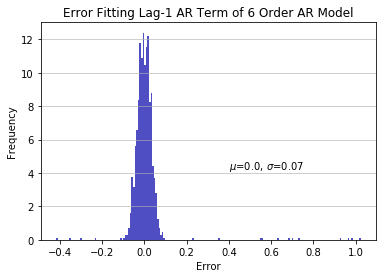
\includegraphics[width=.85\linewidth]{images/ARModelARLag1CoefDist.png}
	\end{figure}

	\begin{figure}[!ht]
		\centering
		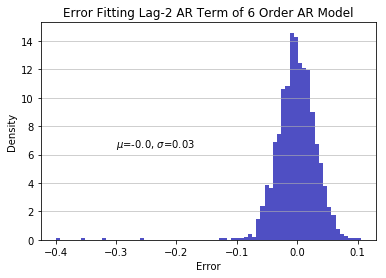
\includegraphics[width=.85\linewidth]{images/ARModelARLag2CoefDist.png}
	\end{figure}
	\begin{figure}[!ht]
		\centering
		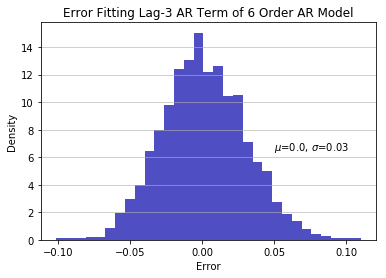
\includegraphics[width=.85\linewidth]{images/ARModelARLag3CoefDist.png}
	\end{figure}
	
	\begin{figure}[!ht]
		\centering
		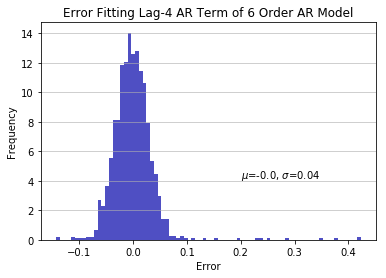
\includegraphics[width=.85\linewidth]{images/ARModelARLag4CoefDist.png}
	\end{figure}
	\begin{figure}[!ht]
		\centering
		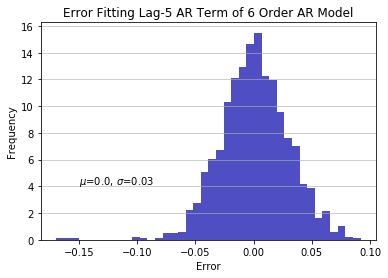
\includegraphics[width=.85\linewidth]{images/ARModelARLag5CoefDist.png}
	\end{figure}
	
	\begin{figure}[!ht]
		\centering
		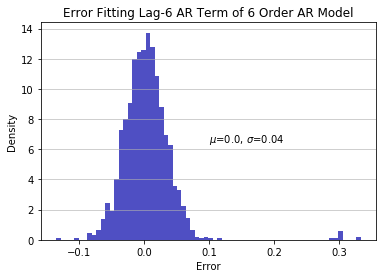
\includegraphics[width=.85\linewidth]{images/ARModelARLag6CoefDist.png}
	\end{figure}

	\begin{figure}[!ht]
		\centering
		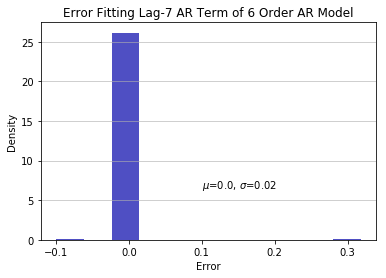
\includegraphics[width=.85\linewidth]{images/ARModelARLag7CoefDist.png}
	\end{figure}
	
	\begin{figure}[!ht]
		\centering
		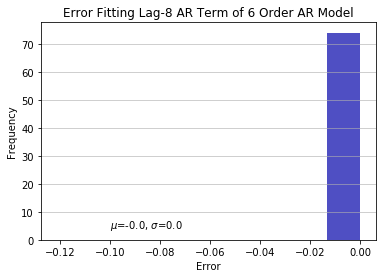
\includegraphics[width=.85\linewidth]{images/ARModelARLag8CoefDist.png}
	\end{figure}

	\begin{figure}[!ht]
		\centering
		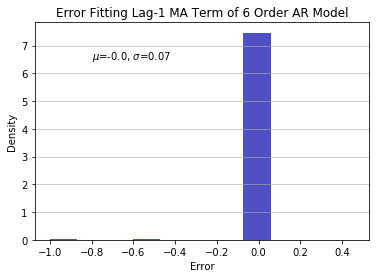
\includegraphics[width=.85\linewidth]{images/ARModelMALag1CoefDist.png}
	\end{figure}
	
	\begin{figure}[!ht]
		\centering
		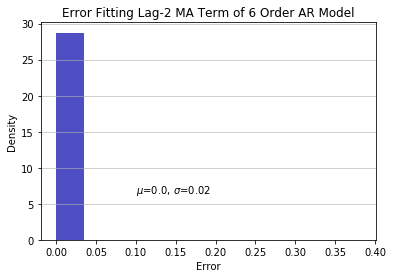
\includegraphics[width=.85\linewidth]{images/ARModelMALag2CoefDist.png}
	\end{figure}


	\begin{figure}[!ht]
		\centering
		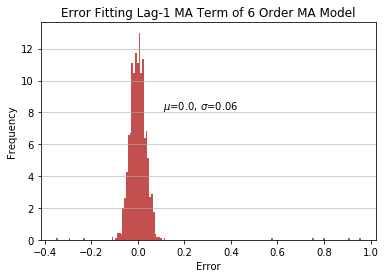
\includegraphics[width=.85\linewidth]{images/MAModelMALag1CoefDist.png}
	\end{figure}
	
	\begin{figure}[!ht]
		\centering
		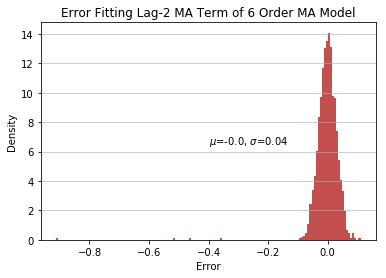
\includegraphics[width=.85\linewidth]{images/MAModelMALag2CoefDist.png}
	\end{figure}
	\begin{figure}[!ht]
		\centering
		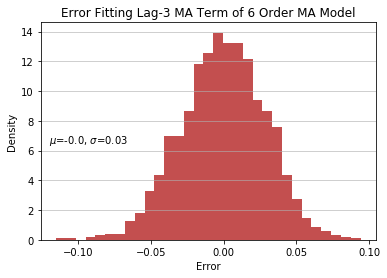
\includegraphics[width=.85\linewidth]{images/MAModelMALag3CoefDist.png}
	\end{figure}
	
	\begin{figure}[!ht]
		\centering
		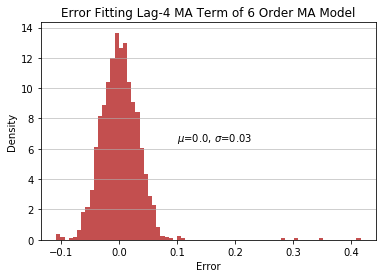
\includegraphics[width=.85\linewidth]{images/MAModelMALag4CoefDist.png}
	\end{figure}
	\begin{figure}[!ht]
		\centering
		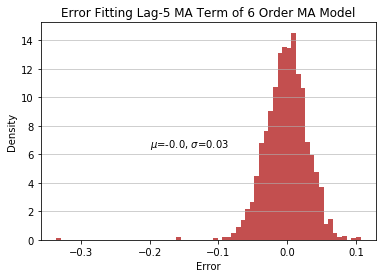
\includegraphics[width=.85\linewidth]{images/MAModelMALag5CoefDist.png}
	\end{figure}
	
	\begin{figure}[!ht]
		\centering
		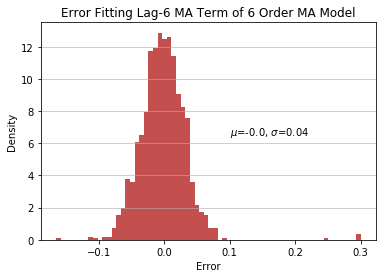
\includegraphics[width=.85\linewidth]{images/MAModelMALag6CoefDist.png}
	\end{figure}
	\begin{figure}[!ht]
		\centering
		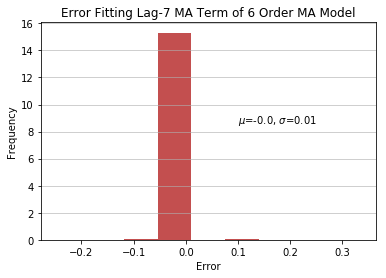
\includegraphics[width=.85\linewidth]{images/MAModelMALag7CoefDist.png}
	\end{figure}
	
	\begin{figure}[!ht]
		\centering
		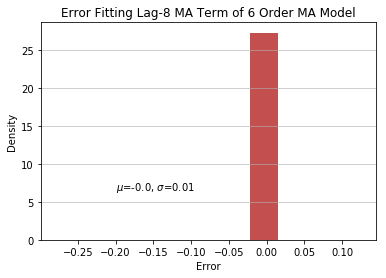
\includegraphics[width=.85\linewidth]{images/MAModelMALag8CoefDist.png}
	\end{figure}
	\begin{figure}[!ht]
		\centering
		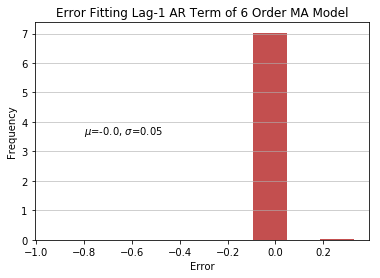
\includegraphics[width=.84\linewidth]{images/MAModelARLag1CoefDist.png}
	\end{figure}
	
	\begin{figure}[!ht]
		\centering
		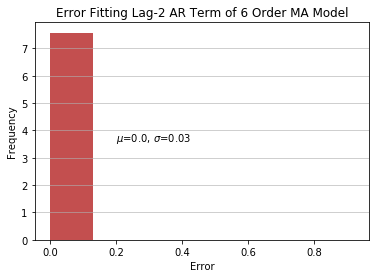
\includegraphics[width=.84\linewidth]{images/MAModelARLag2CoefDist.png}
	\end{figure}
	
\end{document}
